\documentclass[11pt,letterpaper]{article}
\usepackage[T1]{fontenc}
\usepackage[utf8]{inputenc}
\usepackage{lmodern}
\usepackage[margin=0.82in,top=0.75in,bottom=0.78in,headheight=15pt]{geometry}
\usepackage{microtype}
\usepackage{amsmath,amssymb,mathtools}
\usepackage{booktabs,tabularx,array}
\usepackage{graphicx,xcolor}
\usepackage{tikz}
\usetikzlibrary{arrows.meta,positioning,calc}
\usepackage{enumitem}
\usepackage{fancyhdr,lastpage}
\usepackage{titlesec}
\usepackage{xurl}
\usepackage[hidelinks,bookmarksopen=true]{hyperref}
\definecolor{ink}{HTML}{152B3C}
\definecolor{accent}{HTML}{185F76}
\definecolor{pale}{HTML}{F0F5F7}
\definecolor{rule}{HTML}{CED9DF}
\hypersetup{pdftitle={Explicit versus learned search},pdfauthor={Angel Raychev},pdfsubject={Technical retrospective on neural-guided tree search and search-trace learning},pdfkeywords={MCTS,language models,Stream of Search,value learning,search distillation}}
\pagestyle{fancy}
\fancyhf{}
\fancyhead[L]{\small\sffamily\color{ink}Explicit versus learned search}
\fancyhead[R]{\small\sffamily\color{ink}Technical retrospective}
\fancyfoot[L]{\footnotesize Angel Raychev}
\fancyfoot[R]{\footnotesize \thepage\ / \pageref*{LastPage}}
\renewcommand{\headrulewidth}{0.3pt}
\renewcommand{\footrulewidth}{0pt}
\setlength{\parindent}{0pt}
\setlength{\parskip}{6.5pt}
\setlength{\emergencystretch}{2em}
\widowpenalty=10000
\clubpenalty=10000
\setcounter{secnumdepth}{2}
\titleformat{\section}{\Large\sffamily\bfseries\color{ink}}{\thesection}{0.65em}{}
\titleformat{\subsection}{\large\sffamily\bfseries\color{ink}}{\thesubsection}{0.65em}{}
\titlespacing*{\section}{0pt}{18pt}{8pt}
\titlespacing*{\subsection}{0pt}{11pt}{4pt}
\setlist[itemize]{leftmargin=1.3em,itemsep=3pt,topsep=4pt}
\setlist[enumerate]{leftmargin=1.6em,itemsep=3pt,topsep=4pt}
\newcolumntype{Y}{>{\raggedright\arraybackslash}X}
\newcommand{\repo}{\href{https://github.com/RaychevAngel/classical_vs_contextual_search}{companion repository}}
\newcommand{\src}[2]{\href{https://github.com/RaychevAngel/classical_vs_contextual_search/blob/1a7fda10617d34ccd3a87c825cba71e4429de91a/#1}{\texttt{#2}}}
\newcommand{\smallnote}[1]{{\small\color{ink}#1}}
\newcommand{\takeaway}[1]{\par\smallskip\noindent\colorbox{pale}{\parbox{\dimexpr\linewidth-2\fboxsep\relax}{\small\textbf{Key distinction.} #1}}\par\smallskip}
\tikzset{box/.style={draw=rule,fill=pale,rounded corners=2pt,align=center,font=\small\sffamily,inner sep=7pt},flow/.style={-{Stealth[length=2.2mm]},thick,draw=accent},back/.style={-{Stealth[length=2mm]},dashed,draw=accent},label/.style={font=\footnotesize\sffamily,align=center,text=ink}}
\begin{document}
\thispagestyle{empty}
{\huge\sffamily\bfseries\color{ink}Explicit versus learned search\par}
\vspace{5pt}
{\Large\sffamily\color{accent}Neural-guided tree search and search-trace learning\par}
\vspace{13pt}
{\large Angel Raychev\par}
\smallskip
{\small A technical retrospective on joint 2025 work with Yalcin Tur and Mihajlo Stojkovic.\par}
{\small Prepared 23 October 2026\quad\textbullet\quad\href{https://angelraychev.com/explicit-versus-learned-search/}{angelraychev.com}\par}
\vspace{11pt}
\textbf{Overview.} A language model can participate in search in two different ways: an external program can maintain a tree and ask learned models which branches to expand, or a model can learn to represent exploration inside its own generated sequence. I built a research pipeline connecting these approaches: batched neural-guided tree search, iterative policy and value training, and supervised learning from serialized search traversals. The common intermediate object is a search tree; different projections of that tree become different learning signals.

This report explains the implementation and the questions it was designed to investigate. The design centers on the controller/state boundary, the separation of proposal and evaluation, the three tree-to-training data contracts, and the alignment between step-level value targets and model outputs. Those interfaces determine what a comparison between explicit and learned search actually measures.

\smallnote{Scope: this is my retrospective, not a new joint manuscript or a new empirical study. It preserves the credit and identity of the original Stanford CS224N and CS224R projects. No new model training or evaluation was performed for this document. Historical methods are described from the original reports and source; refreshed reuse tooling is distinguished from historical experimental evidence.}

\section{The question is where search happens}
Both approaches use neural networks. ``Explicit'' does not mean non-neural, and ``learned'' does not mean that the alternative has no learned components. The operational contrast is where branching decisions and revisitable state live.

\begin{figure}[ht]
\centering
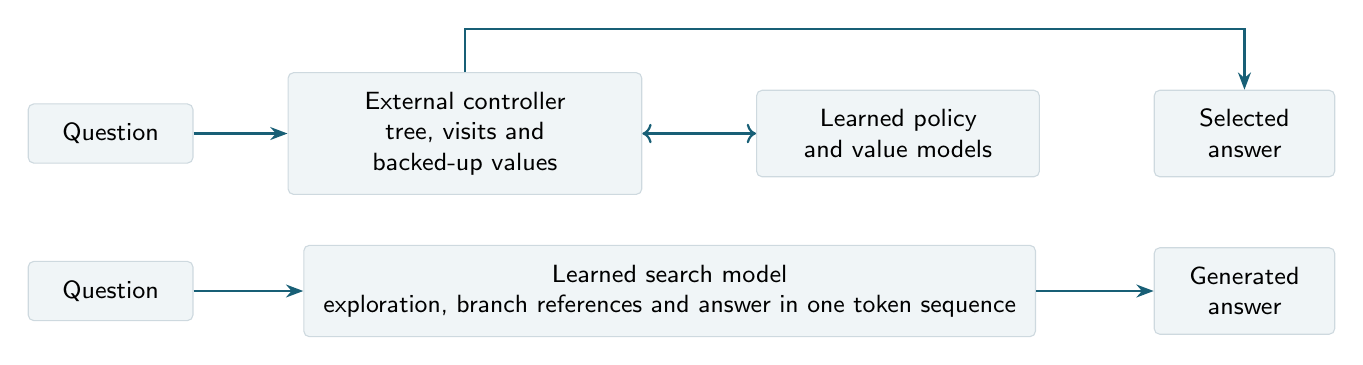
\begin{tikzpicture}[x=1cm,y=1cm]
\node[box,text width=1.6cm] (q1) at (0.6,0) {Question};
\node[box,text width=4.0cm] (tree) at (5.1,0) {External controller\\tree, visits and backed-up values};
\node[box,text width=3.1cm] (models) at (10.6,0) {Learned policy\\and value models};
\node[box,text width=1.8cm] (a1) at (15.0,0) {Selected\\answer};
\draw[flow] (q1)--(tree);
\draw[flow,<->] (tree)--(models);
\draw[flow] (tree.north)--++(0,0.55)-|(a1.north);
\node[box,text width=1.6cm] (q2) at (0.6,-2.0) {Question};
\node[box,text width=8.8cm] (trace) at (7.7,-2.0) {Learned search model\\exploration, branch references and answer in one token sequence};
\node[box,text width=1.8cm] (a2) at (15.0,-2.0) {Generated\\answer};
\draw[flow] (q2)--(trace);
\draw[flow] (trace)--(a2);
\end{tikzpicture}
\caption{Two locations for search control and state. The upper answer is selected by the controller using model-guided statistics; the lower answer is emitted by the search-trace-trained model.}
\label{fig:contrast}
\end{figure}

An external controller explicitly stores alternatives and statistics. A search-trace model represents exploration through text in a finite context. Learning can transfer work from repeated online search into model parameters, but the training examples themselves may require substantial teacher-search computation. The useful comparison therefore concerns a joint allocation of model capacity, training effort and inference effort, not an isolated count of final-answer tokens.

\section{Task representation and information boundaries}
The project used arithmetic construction problems because the inputs, actions and final-answer conditions can be stated precisely. The earlier CS224N study used Game of 24; the later CS224R work generalized the target. A problem can be written
\begin{equation}
q=(X,t),\qquad X=\{x_1,x_2,x_3,x_4\}_{\mathrm{multiset}},
\end{equation}
where a final expression must use each supplied number with its given multiplicity and evaluate to the target $t$ using the permitted operations. The multiset matters: two occurrences of $3$ are two resources, not one distinct value.

The language model proposes a textual step, rather than selecting from a hard-coded enumeration of all legal moves. For a question $q$ and previous actions $a_1,\ldots,a_k$, the model-facing state is the textual prefix
\begin{equation}
s_k=(q,a_1,\ldots,a_k),\qquad a_{k+1}\sim\pi_\theta(\,\cdot\mid s_k).
\end{equation}
An action might combine two remaining numbers and report the remainder. A separate final-answer marker identifies a terminal proposal.

\begin{center}
\begin{minipage}{0.94\linewidth}
\small\ttfamily
Use 3, 3, 5, 12 to make 51.\par
3*12=36 Left: 3, 5, 36\par
3*5=15 Left: 15, 36\par
36+15=51 Left: 51\par
The answer is: 3*12+3*5=51.
\end{minipage}
\end{center}
\smallnote{Worked arithmetic illustration. This is not a new sampled rollout or a measured result. The same problem appears in the original search-trace example.}

\subsection{A learned value is not a correctness certificate}
The value model estimates the promise of a prefix. It does not prove that the prefix's arithmetic or state bookkeeping is legal. In the historical implementation, partial states were model-generated text, and the terminal expression was checked separately. Describing the environment as precisely specifiable must not be confused with claiming that every intermediate step was enforced by a symbolic transition engine.

The distinction also separates two outcomes:
\begin{align}
\text{discovery success}&:\quad\exists\text{ a correct terminal candidate in the explored tree},\\
\text{selection success}&:\quad\text{the method's chosen final answer is correct}.
\end{align}
The first asks whether exploration found a solution. The second additionally tests whether the method recognized and selected it. Using an answer checker to choose a final candidate would change the information available to the method.

\subsection{Training and evaluation have different roles for the checker}
For data generation, terminal outcomes supply labels and identify successful trajectories for training. For the historical MCTS evaluation path, learned values guide search and terminal backups; the controller selects an answer before the final checker scores it. There is no basis for describing this evaluation path as an oracle that simply returns whichever explored answer is correct.

\takeaway{The environment supplies a task and a final correctness condition. The policy proposes, the value model estimates, the controller searches and selects, and the evaluator measures. These are distinct responsibilities even when they share data structures.}

\section{A custom policy--value search controller}
The search engine stores a node's textual state, parent and children, visit count $N$, backed-up action value $Q$, and initial learned estimate $v_\phi$. The policy and value model are separate services. The policy generates candidate continuations; the value model scores the resulting child prefixes. This separation permits independent model choices and training updates.

\subsection{Selection, expansion and backup}
The selection rule implemented in the inspected 2025 controller is
\begin{equation}
u^*=\operatorname*{arg\,max}_{u\in\mathrm{children}(s)}
\left[Q(u)+c\,\frac{\sqrt{N(s)}}{N(u)+1}\right].
\label{eq:selection}
\end{equation}
Here $c$ controls exploration. The policy supplies sampled children, not a policy-prior multiplier in this formula. This is an AlphaZero-inspired system, not an exact reproduction of AlphaZero or canonical PUCT.

At an expansion, the policy supplies up to the configured branch factor $b$ of candidate continuations. The adapter appends each candidate to its parent prefix and evaluates all resulting children with $v_\phi$. New children start with zero visits and their learned estimate as the initial action value. A traversal backs a scalar $z$ up the ancestry through running means:
\begin{equation}
N(s)\leftarrow N(s)+1,\qquad
Q(s)\leftarrow Q(s)+\frac{z-Q(s)}{N(s)}.
\label{eq:backup}
\end{equation}
The source of $z$ matters: learned estimates evaluate nonterminal states; terminal outcomes supply data-generation labels. The evaluation subclass instead backs up learned terminal estimates. Shared tree machinery thus supports different collection and measurement semantics without an answer-selection oracle.

The implementation searches up to configured expansion budgets and can return results at multiple budget checkpoints while continuing the same tree. At the end, it follows maximum-$Q$ children to a leaf. That actual final-choice rule is distinct from the exploration rule in Equation~\eqref{eq:selection} and from a most-visited-child rule.

\subsection{The adapter is part of the algorithmic contract}
A model interface returns candidate states paired with values. It batches policy requests, flattens children for value inference and maps replies back to each parent. Model serving and tree statistics remain separate responsibilities.

The interface separates proposal quality and diversity from value quality; policy capacity from evaluator capacity; branching breadth from expansion count; and local model scores from the controller's accumulated evidence.
More children also create more evaluation work. A value model can misrank a correct continuation. Extra search effort is not useful progress by definition; the complete system must be measured.

\smallnote{Implementation anchors: \src{utils/mcts_base.py}{utils/mcts\_base.py}, \src{utils/policy_value.py}{utils/policy\_value.py}, and \src{evaluate/mcts_evaluator.py}{evaluate/mcts\_evaluator.py}. These links point to the historical source snapshot, not to an unrecorded moving branch.}

\section{Batching a forest instead of waiting on one tree}
Individual searches have irregular control flow: one prefix needs expansion, another is waiting for a response, and a third has reached a terminal answer. Running each question as a completely isolated sequence of tiny model requests would couple inference efficiency to that irregularity. The forest abstraction collects expansion work from many trees into a common queue.

\begin{figure}[ht]
\centering
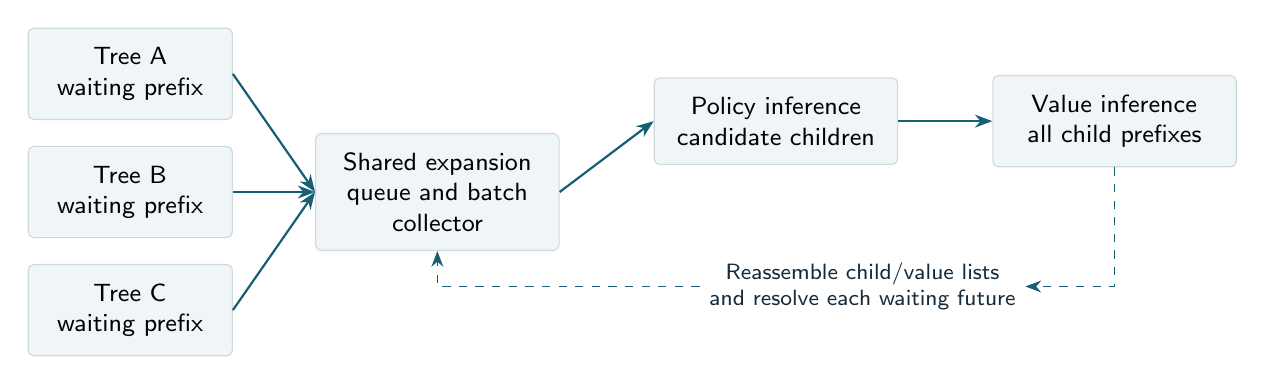
\begin{tikzpicture}[x=1cm,y=1cm]
\node[box,text width=2.1cm] (t1) at (1.1,0) {Tree A\\waiting prefix};
\node[box,text width=2.1cm] (t2) at (1.1,-1.5) {Tree B\\waiting prefix};
\node[box,text width=2.1cm] (t3) at (1.1,-3.0) {Tree C\\waiting prefix};
\node[box,text width=2.6cm] (queue) at (5.0,-1.5) {Shared expansion\\queue and batch\\collector};
\node[box,text width=2.6cm] (policy) at (9.3,-0.6) {Policy inference\\candidate children};
\node[box,text width=2.6cm] (value) at (13.6,-0.6) {Value inference\\all child prefixes};
\node[label] (reply) at (10.4,-2.7) {Reassemble child/value lists\\and resolve each waiting future};
\draw[flow] (t1.east)--(queue.west);
\draw[flow] (t2.east)--(queue.west);
\draw[flow] (t3.east)--(queue.west);
\draw[flow] (queue.east)--(policy.west);
\draw[flow] (policy.east)--(value.west);
\draw[back] (value.south)|-(reply.east);
\draw[back] (reply.west)-|(queue.south);
\end{tikzpicture}
\caption{The forest converts independent search-control flows into batched policy and value work, then returns each result to the tree that requested it.}
\label{fig:forest}
\end{figure}

Each tree enqueues a question/prefix pair with a future. The collector forms batches, calls the policy--value adapter and routes each returned list to the matching future. Tree slots then continue traversal or pick up another question. The source allocates tree slots separately from model batch size (specifically, twice that batch size), so the forest can hold more waiting searches than fit in one inference batch.

There are two distinct batching operations. First, several parent prefixes are presented to the policy together. Second, all sampled children from those prefixes are flattened into a value batch. The latter batch may be substantially larger than the former. Reassembly preserves the correspondence between each parent, its proposed children and their estimates.

\subsection{Scheduling, batching and hardware utilization}
The forest uses asynchronous tasks and futures to express independent tree progress, while the historical service adapter uses synchronous HTTP calls. Batching is explicit; hardware throughput and network overlap are separate execution properties to measure.

The pipeline has an explicit unit of scheduling: an expansion request, rather than an entire problem or an individual output token. It also separates three things often collapsed into ``batch size'': the number of live questions, the number of parent prefixes in a model call, and the number of child prefixes to be evaluated.

The broader reusable pattern is a queue between irregular control flow and regular batched inference. The same idea is relevant whenever an agent's next action depends on previous results, while the expensive neural operations benefit from grouping work across independent tasks.

\section{One tree produces three training datasets}
The search tree is not only an inference artifact. The generator projects it into three different supervised products. Keeping those products explicit is one of the most useful parts of the implementation: they preserve different information and should not be described as interchangeable ``synthetic data.''

\begin{figure}[ht]
\centering
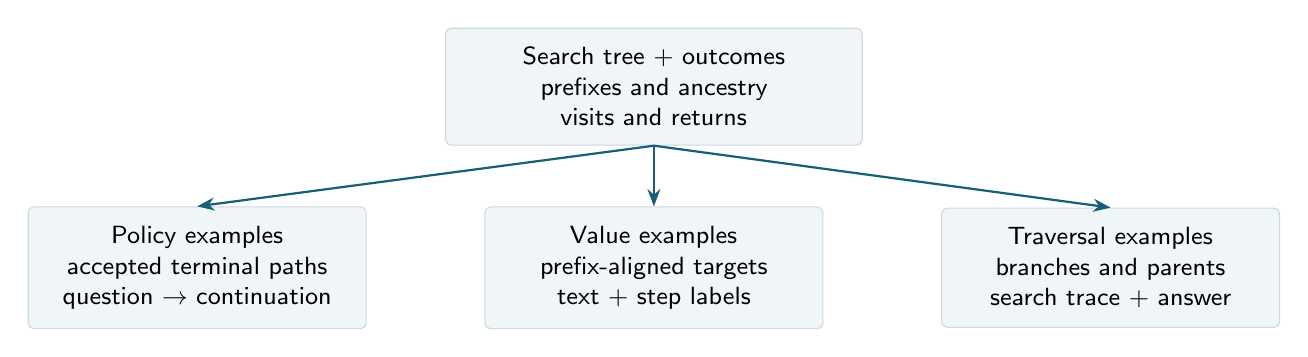
\begin{tikzpicture}[x=1cm,y=1cm]
\node[box,text width=4.8cm] (tree) at (7.4,0) {Search tree + outcomes\\prefixes and ancestry\\visits and returns};
\node[box,text width=3.8cm] (p) at (1.6,-2.3) {Policy examples\\accepted terminal paths\\question $\to$ continuation};
\node[box,text width=3.8cm] (v) at (7.4,-2.3) {Value examples\\prefix-aligned targets\\text + step labels};
\node[box,text width=3.8cm] (s) at (13.2,-2.3) {Traversal examples\\branches and parents\\search trace + answer};
\draw[flow] (tree.south)--(p.north);
\draw[flow] (tree.south)--(v.north);
\draw[flow] (tree.south)--(s.north);
\end{tikzpicture}
\caption{Three projections of the same search process. A successful path teaches a continuation; a return-labeled prefix teaches an estimate; a traversal teaches how exploration is represented.}
\label{fig:products}
\end{figure}

\begin{table}[ht]
\small\centering
\begin{tabularx}{\linewidth}{@{}p{0.14\linewidth}YY@{}}
\toprule
Product & Stored contract & Information retained \\
\midrule
Policy & Question and full accepted terminal continuation & A successful path, including its textual steps and final expression. \\
Value & Question plus trajectory text, with an ordered label list & Targets aligned to the question/step boundaries along each terminal path. \\
Traversal & Question, first-visit trace and selected accepted answer & Alternative branches, explicit node/parent identifiers and a final answer. \\
\bottomrule
\end{tabularx}
\end{table}

\subsection{Policy learning from accepted paths}
Let $\mathcal D_+$ contain terminal trajectories accepted by the collection-time checker. The policy objective is ordinary supervised next-token learning on those trajectories:
\begin{equation}
\mathcal L_{\mathrm{policy}}(\theta)
=-\mathbb E_{(q,\tau)\sim\mathcal D_+}\log\pi_\theta(\tau\mid q).
\end{equation}
The selection mechanism matters: these are paths discovered by the current search process, not samples from an independently specified optimal-policy distribution. Updating the models changes which paths the next collection round is likely to produce. The implementation thus connects search-assisted data collection to iterative supervised improvement.

Before iterative search-assisted training, synthetic worked examples bootstrap the policy's step format and final-answer convention. That initial supervised stage gives the search controller a usable proposal interface; subsequent rounds replace fixed formatting examples with successful paths discovered by the evolving policy--value system.

\subsection{Value targets summarize observed returns}
For a node $s$, let $\mathcal R(s)$ be the multiset of terminal returns actually backed up through it during data collection. When that multiset is nonempty, the generator uses
\begin{equation}
\widehat v(s)=\frac{1}{|\mathcal R(s)|}\sum_{r\in\mathcal R(s)}r.
\label{eq:target}
\end{equation}
It falls back to the current terminal path's label when no backed-up labels are present. Consequently, intermediate labels can be fractional even though each terminal outcome is binary. They are search- and visitation-dependent empirical targets, not true optimal values or exhaustive averages over every reachable solution.

\subsection{Step-value learning without replacing the language-model head}
The later implementation makes the label/output alignment concrete. It retains a causal language model's vocabulary head, takes the logit corresponding to the token \texttt{1}, and trains that scalar with a binary-cross-entropy objective. If $\ell_\phi(s_j)$ is that designated logit at a labeled boundary, then
\begin{equation}
v_\phi(s_j)=\sigma\!\left(\ell_\phi(s_j)\right),\qquad
\mathcal L_{\mathrm{value}}=
\frac{1}{\sum_j m_j}\sum_j m_j\,\operatorname{BCEWithLogits}
\left(\ell_\phi(s_j),y_j\right),
\label{eq:value}
\end{equation}
where $m_j$ selects supervised boundary positions and $y_j$ is the corresponding return target. This is a sigmoid of one vocabulary logit, not the softmax probability that the model would generate the token \texttt{1}.

The tokenizer identifies tokens whose decoded text contains a newline. The dataset transformation aligns the ordered label list to those positions. Nonlabel tokens and padding receive a sentinel value and are masked out of the loss. The model wrapper checks that the newline mask and label mask agree, rather than silently training against shifted or missing labels.

At inference, the value service takes the same designated vocabulary logit at the end of a supplied prefix and applies a sigmoid. Keeping the value readout inside the ordinary language-model head makes the later value model compatible with the vLLM-based serving path. The important design is the agreement among data boundaries, loss mask, readout position and inference-time extraction.

\subsection{Two historical stages, not one interchangeable configuration}
The project evolved between the two Stanford reports. Their task distributions, model families and value implementations must remain distinguishable.

\begin{table}[ht]
\small
\begin{tabularx}{\linewidth}{@{}p{0.18\linewidth}YY@{}}
\toprule
 & CS224N stage & CS224R stage \\
\midrule
Task & Game of 24 & Generalized arithmetic target \\
Model framing & SmolLM2 policy/value size combinations & Qwen-based policy/value search and a separate search-trace model \\
Value readout & A custom scalar head described in the original report & A designated vocabulary logit, sigmoid and masked step-level training in the later source \\
Learning focus & Iterative policy/value data generation and capacity/allocation sweeps & Search-to-policy/value/traversal data, followed by search-trace learning and self-training \\
\bottomrule
\end{tabularx}
\caption{Methodological continuity does not make the two experimental setups identical. These descriptions identify the historical stages; they are not a new matched performance comparison.}
\end{table}

The CS224N report describes a separate nonlinear value head served with PyTorch/FastAPI. The later vocabulary-logit approach supports a different serving path. Architecture, checkpoints and results should be attributed to the appropriate stage.

\smallnote{Implementation anchors: \src{generate_data/mcts_generator.py}{generator}, \src{train/value_trainer.py}{step-value trainer}, \src{utils/deployer_value.py}{value server} and \src{train/policy_trainer.py}{policy trainer}.}

\section{Learning a search traversal, not only its successful path}
A successful trajectory omits the alternatives that were considered along the way. Stream-of-Search-style supervision retains more of that process: the generator records nodes in first-visit order and serializes references to their parents or ancestry. A model can then be trained on text that contains branch switching, unsuccessful avenues and a selected final answer.

\begin{samepage}
For the running arithmetic example, successful and unsuccessful branches can coexist:
\begin{center}
\begin{minipage}{0.94\linewidth}
\small\ttfamily
Q | Use 3, 3, 5, 12 to make 51.\par
<START\_THOUGHT>\par
N1->Q | 3*12=36 Left: 3, 5, 36\par
N2->Q | 12*5=60 Left: 3, 3, 60\par
N3->N1 | 3*5=15 Left: 15, 36\par
N4->N2 | 3*3=9 Left: 9, 60\par
N5->N3 | 36+15=51 Left: 51\par
N6->N4 | 60-9=51 Left: 51\par
N7->N2 | 60-3=57 Left: 3, 57\par
N8->N7 | 57-3=54 Left: 54\par
<END\_THOUGHT>\par
<START\_ANSWER>\par
3*12+3*5=51\par
<END\_ANSWER>
\end{minipage}
\end{center}
\smallnote{Simplified illustrative serialization, not a new model output or an exact byte-for-byte saved traversal. The generator's terminal entries may include the full ancestor chain. Two branches reach 51; the branch through \texttt{N7} and \texttt{N8} reaches 54 instead, preserving an unsuccessful avenue alongside the selected answer.}
\end{samepage}

The parent identifiers make the distinction from a linear solution explicit. Node \texttt{N4} continues \texttt{N2}, not the immediately preceding textual line \texttt{N3}. The next generated token can therefore describe an action in a different branch while the sequence as a whole remains linear.

\subsection{What the supervision asks the model to absorb}
The traversal model is fine-tuned on teacher-search traces and answers. It starts from a pretrained language model; ``a fresh model'' here does not mean training randomly initialized weights. The target is a representation of the teacher's exploration process, including its ordering and branch references, rather than a guarantee that every teacher decision is optimal.

Search-trace learning can amortize the cost of exploration across future questions. It may also inherit the teacher's limitations and the trace distribution's conventions. More trace tokens are not automatically more useful supervision: branch diversity, the recoverability of state, sequence length and the quality of the appended answer all influence what can be learned.

\subsection{Rejection self-training after traversal supervision}
The project also implements a STaR-style self-training path: generate candidate completions on new questions, retain accepted completions and use them in a subsequent training dataset. The scripts can revisit unresolved questions over repeated generation rounds. That is a concrete generate--verify--train loop; it should not be equated with every detail of the original STaR algorithm, including its answer-conditioned rationalization step~\cite{star}.

The external controller and the learned traversal model are therefore connected by more than a shared benchmark. Search builds a teacher distribution; serialization determines what the student sees; supervised learning and rejection self-training determine how that experience is absorbed into later generation.

\section{What the experiments were designed to investigate}
The original work explored interactions among model capacity, training iteration and inference-time search. Its engineering supports several useful, separable research questions.

\textbf{How should compute be divided between proposing and evaluating?} A stronger policy can supply better candidates; a stronger value model can rank or direct them more effectively. Independent policy/value choices expose that interaction instead of treating ``the model'' as one undifferentiated object.

\textbf{How should exploration be divided between breadth and repeated expansion?} A branch factor changes how many candidates an expansion proposes. The expansion budget changes how much of the tree can be developed. Their product is a rough operation count, not a complete accounting of neural inference cost or of the information that the search actually gains.

\textbf{What does an additional learning round buy?} Repeated collection with updated models changes the next training distribution. A policy may learn more productive continuations; a value model may better distinguish promising prefixes. Those effects must be separated from merely spending additional teacher-search compute.

\textbf{Which aspects of search transfer into a token sequence?} Traversal supervision preserves alternatives and branch references that path-only SFT discards. The important question is not whether the sequence visually resembles deliberation, but whether the learned procedure remains effective as task depth, branching or the available inference budget changes.

\subsection{Accounting that keeps a comparison interpretable}
A model parameter count is not an inference budget. A policy--value pair and a single traversal model can have similar total parameter counts but incur different costs through model calls, prefix lengths, batching and generated tokens. A useful accounting separates
\begin{equation}
C_{\mathrm{total}}(n)=C_{\mathrm{training}}+C_{\mathrm{teacher\ search}}
+\sum_{i=1}^{n}C_{\mathrm{inference}}(q_i).
\end{equation}
This identity is an accounting frame, not a fitted cost model or a reported measurement. It makes amortization explicit: an expensive construction/training process may be worthwhile when reused across many future queries.

For a new controlled study, each comparison should fix or explicitly vary the legal action language, state access, training data, verifier access and final-selection rule. It should record both discovery and selected-answer success, along with policy/value calls, token lengths, elapsed time and context limits. A fixed parameter total or an output-token threshold alone does not equalize those resources.

\subsection{The result this retrospective does and does not assert}
The implemented pipeline and released artifacts establish substantive work on neural-guided search, custom value learning and search-to-training interfaces. This report does not reissue historical accuracy curves as newly verified results, infer a universal winner, or claim an asymptotic capability separation from finite-budget arithmetic experiments. The original reports remain the primary record of their respective studies.

For a finite arithmetic task with complete legal enumeration, exhaustive search can in principle find an existing solution. The scientifically meaningful contrasts concern resource efficiency, learned control, representation and generalization under stated constraints. An empirical plateau is not by itself a proof that a method can never benefit from additional computation.

\section{Artifacts, reuse and contribution}
The \repo{} contains the search engine, policy/value interface, data generator, trainers and experiment scripts. Historical source is linked at the June 2025 snapshot throughout this report. Public policy, value and search-trace model artifacts make the training pipeline inspectable beyond its implementation: readers can inspect experimental weights, configurations and model cards.

The refreshed companion materials separate inspection and reuse from the original study. Clearer instructions, exact arithmetic checking and output accounting do not retroactively rescore old model outputs. Local CPU integrity checks exercise defined data/verification boundaries; model training and evaluation additionally require the appropriate data, model access, serving environment and GPU resources.

\subsection{A compact reproducibility contract}
An interpretable execution record should associate every result with:
\begin{enumerate}
\item the task definition, canonical problem split and exact checker version;
\item immutable policy, value and traversal model revisions, plus tokenizer settings;
\item generation configuration, tree budgets and the final-selection rule;
\item the teacher-search data and the distinct policy/value/traversal projections;
\item actual completed outcomes and denominators, not only a presentation-layer scalar;
\item measured or explicitly approximated training and inference resources.
\end{enumerate}
This is a contract for reusable evidence, not a claim that all historical runs have been reconstructed. No new GPU run was required to document the architecture or to preserve the available sources.

\subsection{My contribution and the original collaboration}
The work began as a joint Stanford CS224N project by Yalcin Tur, Mihajlo Stojkovic and me. The original report credits me with MCTS implementation, evaluation and writing; it credits Yalcin and Mihajlo with policy/value training, data generation and infrastructure for that stage.

I subsequently extended the work for Stanford CS224R. That report identifies me as lead developer, credits most of the later codebase, repeated MCTS refactors and the experiments, and retains Yalcin and Mihajlo's credit for the initial code. My later engineering emphasis was the end-to-end pipeline: efficient batching across searches, iterative model/data flow, step-value training and the search-trace branch. Anjiang Wei and Rafael Rafailov are named as mentors in the CS224N report.

This retrospective is authored by me. The two original reports retain their original authorship and identity.

\takeaway{The reusable idea is to treat search as both an inference procedure and a producer of structured learning signals. Which parts should remain in an external controller, which should be represented in context, and which should be amortized into model parameters is a joint systems-and-learning question.}

\smallskip
\textbf{Resources.} \href{https://angelraychev.com/explicit-versus-learned-search/}{Project article and downloads}; \repo{}; \href{https://huggingface.co/AngelRaychev}{public model artifacts}; and the \href{https://cs224r.stanford.edu/spring_2025/projects/pdfs/CS_224R_Final_Report__3_%20%281%29.pdf}{original Stanford CS224R report}.

\clearpage
\section*{Research context and primary references}
\addcontentsline{toc}{section}{Research context and primary references}
The work sits at the intersection of neural-guided external search and learned representations of search. TS-LLM studies AlphaZero-like tree search for language-model decoding and training~\cite{tsllm}. Stream of Search provides a direct precedent for encoding exploration as a flattened language sequence~\cite{sos}. STaR supplies the broader generate--verify--train self-improvement context~\cite{star}. Schultz and colleagues explicitly contrast external and internal planning with language models in board games~\cite{schultz}. These connections explain the project's framing; this retrospective does not claim that either broad approach was introduced here.

\begin{thebibliography}{9}
\setlength{\itemsep}{8pt}
\bibitem{originaln}
Yalcin Tur, Mihajlo Stojkovic and Angel Raychev.
\emph{Size Doesn't Matter If You Search Enough}. Stanford CS224N custom project report, 2025.

\bibitem{originalr}
Angel Raychev, Yalcin Tur and Mihajlo Stojkovic.
\emph{In-context Search: Efficiency Boost or Fundamentally New Capability?}
Stanford CS224R final report, 2025.
\href{https://cs224r.stanford.edu/spring_2025/projects/pdfs/CS_224R_Final_Report__3_%20%281%29.pdf}{Public Stanford copy}.

\bibitem{code}
Angel Raychev, Yalcin Tur and Mihajlo Stojkovic.
\emph{Classical versus contextual search}. Project source, historical snapshot
\href{https://github.com/RaychevAngel/classical_vs_contextual_search/tree/1a7fda10617d34ccd3a87c825cba71e4429de91a}{\texttt{1a7fda1}}, June 2025; refreshed companion materials available from the \repo{}.

\bibitem{tsllm}
Xidong Feng and colleagues.
\emph{AlphaZero-Like Tree-Search Can Guide Large Language Model Decoding and Training}.
2023. \href{https://arxiv.org/abs/2309.17179}{arXiv:2309.17179}.

\bibitem{sos}
Kanishk Gandhi, Denise Lee, Gabriel Grand, Muxin Liu, Winson Cheng, Archit Sharma and Noah D. Goodman.
\emph{Stream of Search (SoS): Learning to Search in Language}.
2024. \href{https://arxiv.org/abs/2404.03683}{arXiv:2404.03683}.

\bibitem{star}
Eric Zelikman, Yuhuai Wu, Jesse Mu and Noah D. Goodman.
\emph{STaR: Bootstrapping Reasoning With Reasoning}.
2022. \href{https://arxiv.org/abs/2203.14465}{arXiv:2203.14465}.

\bibitem{schultz}
John Schultz and colleagues.
\emph{Mastering Board Games by External and Internal Planning with Language Models}.
2024; revised 2025. \href{https://arxiv.org/abs/2412.12119}{arXiv:2412.12119}.
\end{thebibliography}
\end{document}
